\section{Durchführung}
\label{sec:Durchführung}
Im Versuch sollen die Reichweite von Alphastrahlung und die Statistik des
radioaktiven Zerfalls bestimmt werden. Dazu wird die in Abbildung \ref{fig:geraet}
dargestellte Apparatur verwendet.

\begin{figure}[H]
  \centering
  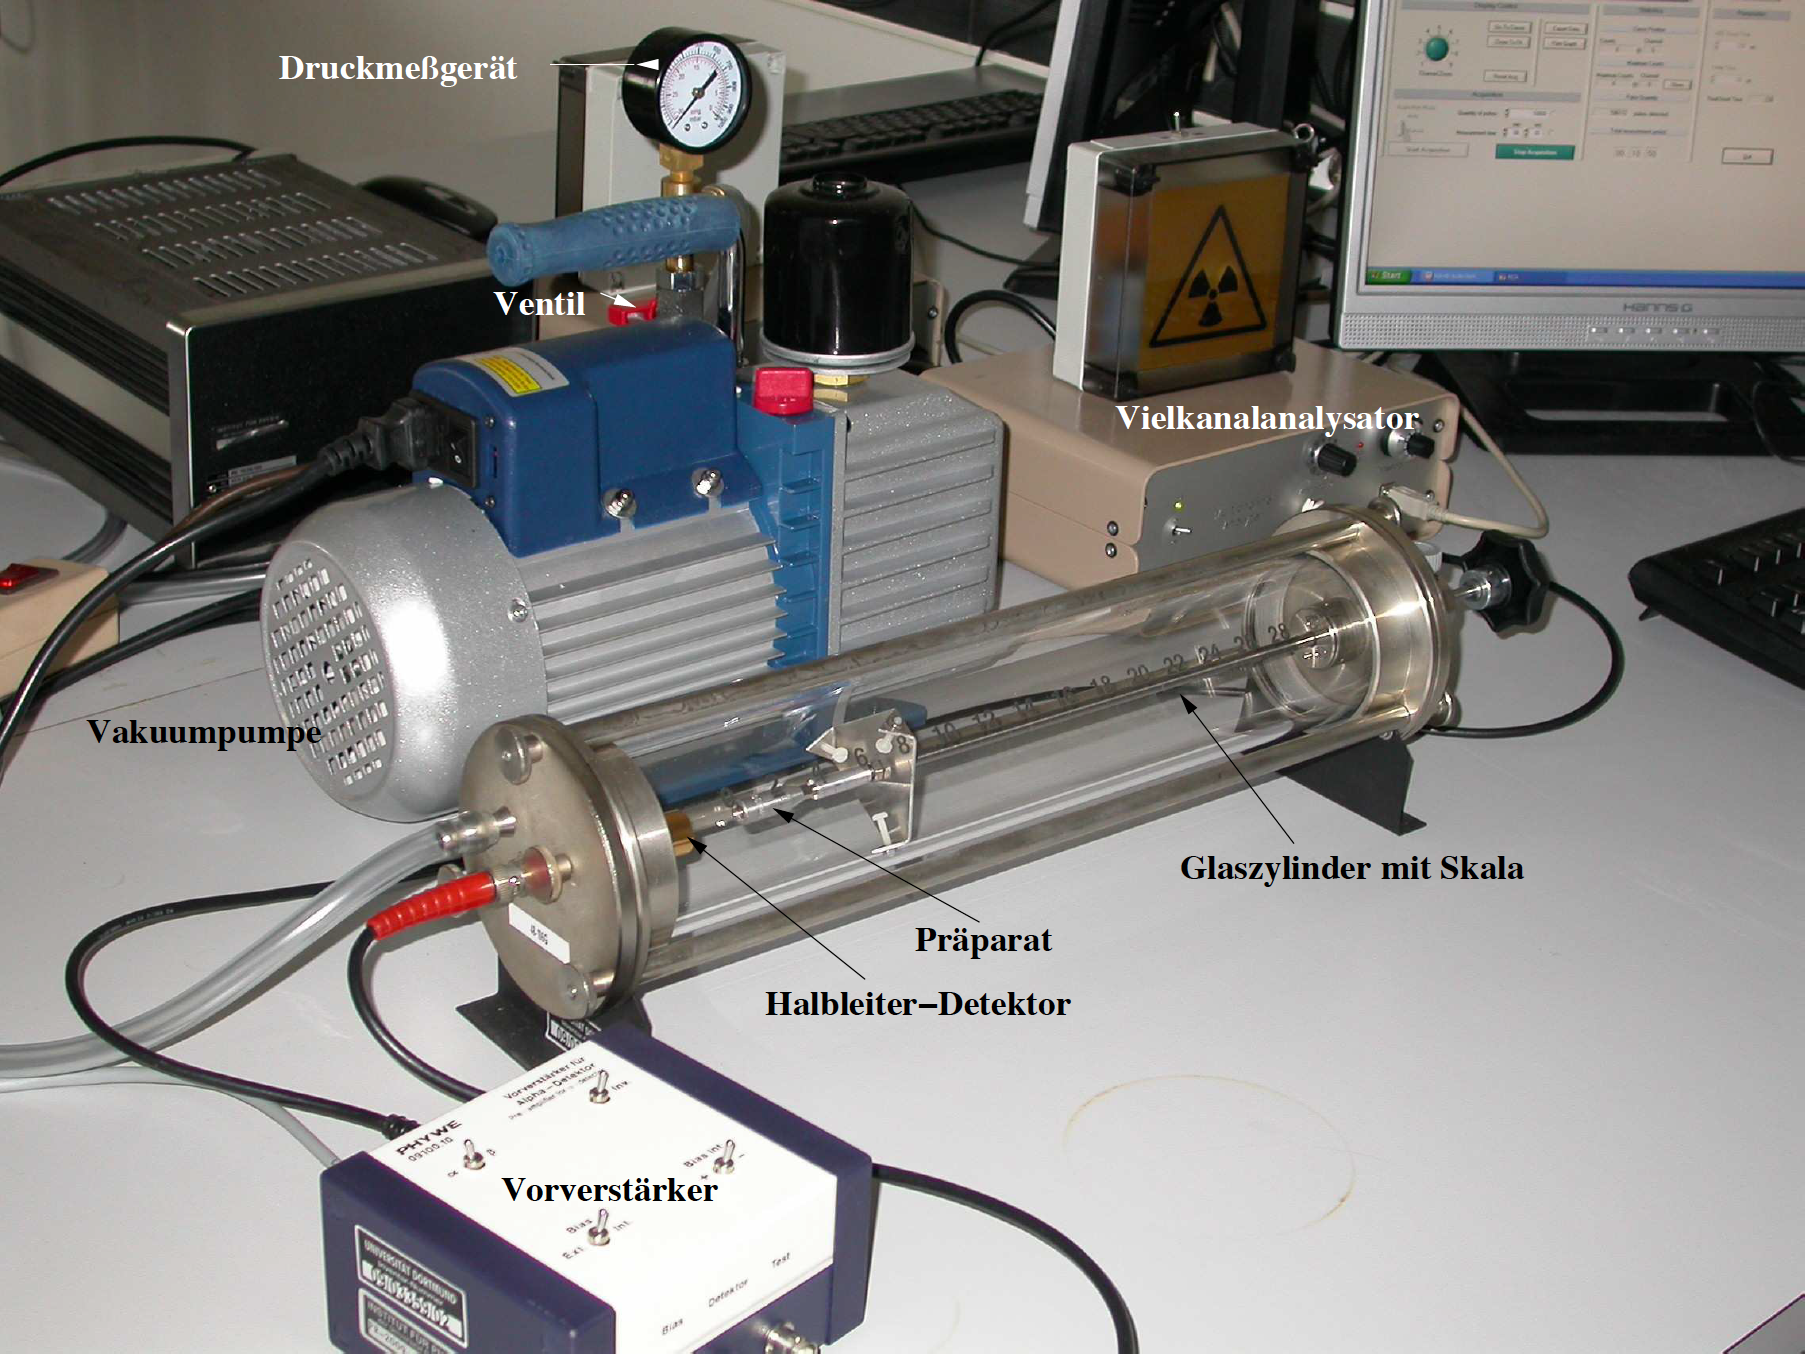
\includegraphics[width=\textwidth]{data/aufbau.png}
  \caption{Skizze der Messapparatur \cite{Versuchsanleitung}.}
  \label{fig:geraet}
\end{figure}

Als Strahlungsquelle wird ein Am-Präparat verwendet. Dieses befindet sich in einem
Glaszylinder, der mithilfe einer Vakuumpumpe evakuiert werden kann. Die Alphastrahlung
wird mithilfe eines Halbleiter-Sperrschichtzählers detektiert. Das Signal desselben ist
an einen Vorverstärker angeschlossen. Das bereits verstärkte Signal wird an einen
Vielkanalanalysator weitergeleitet, der es nach seiner Impulshöhe analysiert. Der
Vielkanalanalysator ist mit einem Computer verbunden, auf dem in einem Programm zur
Messung die benötigten Werte abgelesen werden können.

Um das Grundrauschen bei der Messung zu unterdrücken, muss vor Beginn der Messung
am Vielkanalanalysator eine Diskriminatorschwelle eingestellt werden. Dafür wird
die Strahlungsquelle bei Umgebungsdruck möglichst weit vom Detektor entfernt und
die Diskriminatorschwelle so eingestellt, dass keine Pulse mehr gezählt werden.
Danach wird die Strahlungsquelle so nah an den Detektor gebracht, dass wieder
Pulse gezählt werden. Anschließend wird die Röhre evakuiert und die Messung wird gestartet.

Es wird in Intervallen von 50\, mbar die absolute Anzahl der Pulse und der Channel,
in dem das Maximum der Pulse liegt, in einem Zeitintervall von 120\,s gemessen.

Zur Überprüfung der Statistik des radioaktiven Zerfalls wird in einem Intervall
von 10\,s die Anzahl der registrierten Pulse in der evakuierten Röhre gemessen. Diese
Messung wird 100 mal wiederholt.
